\graphicspath{{figures/analysis/}}
\chapter{Data Analysis}\label{ch:data_anal}
To be able to develop a solution which is able to detect which type of occlusion occurs and the location of it, some analysis of the data is necessary. This is also done to determine how many and which kind of categories of occlusions there are.

\section{Video Capture}
The video used is recorded from above the aquarium with a \gls{nir} backlight which makes the dark zebrafish stand out in contrast to the background. The video is $ 60 $ seconds long with three zebrafish recorded at $ 50 $ \gls{fps} yielding a total of $3000$ frames to be processed. An overview of the recording setup is shown in \autoref{fig:recording}

\begin{figure}[H]
	\centering
	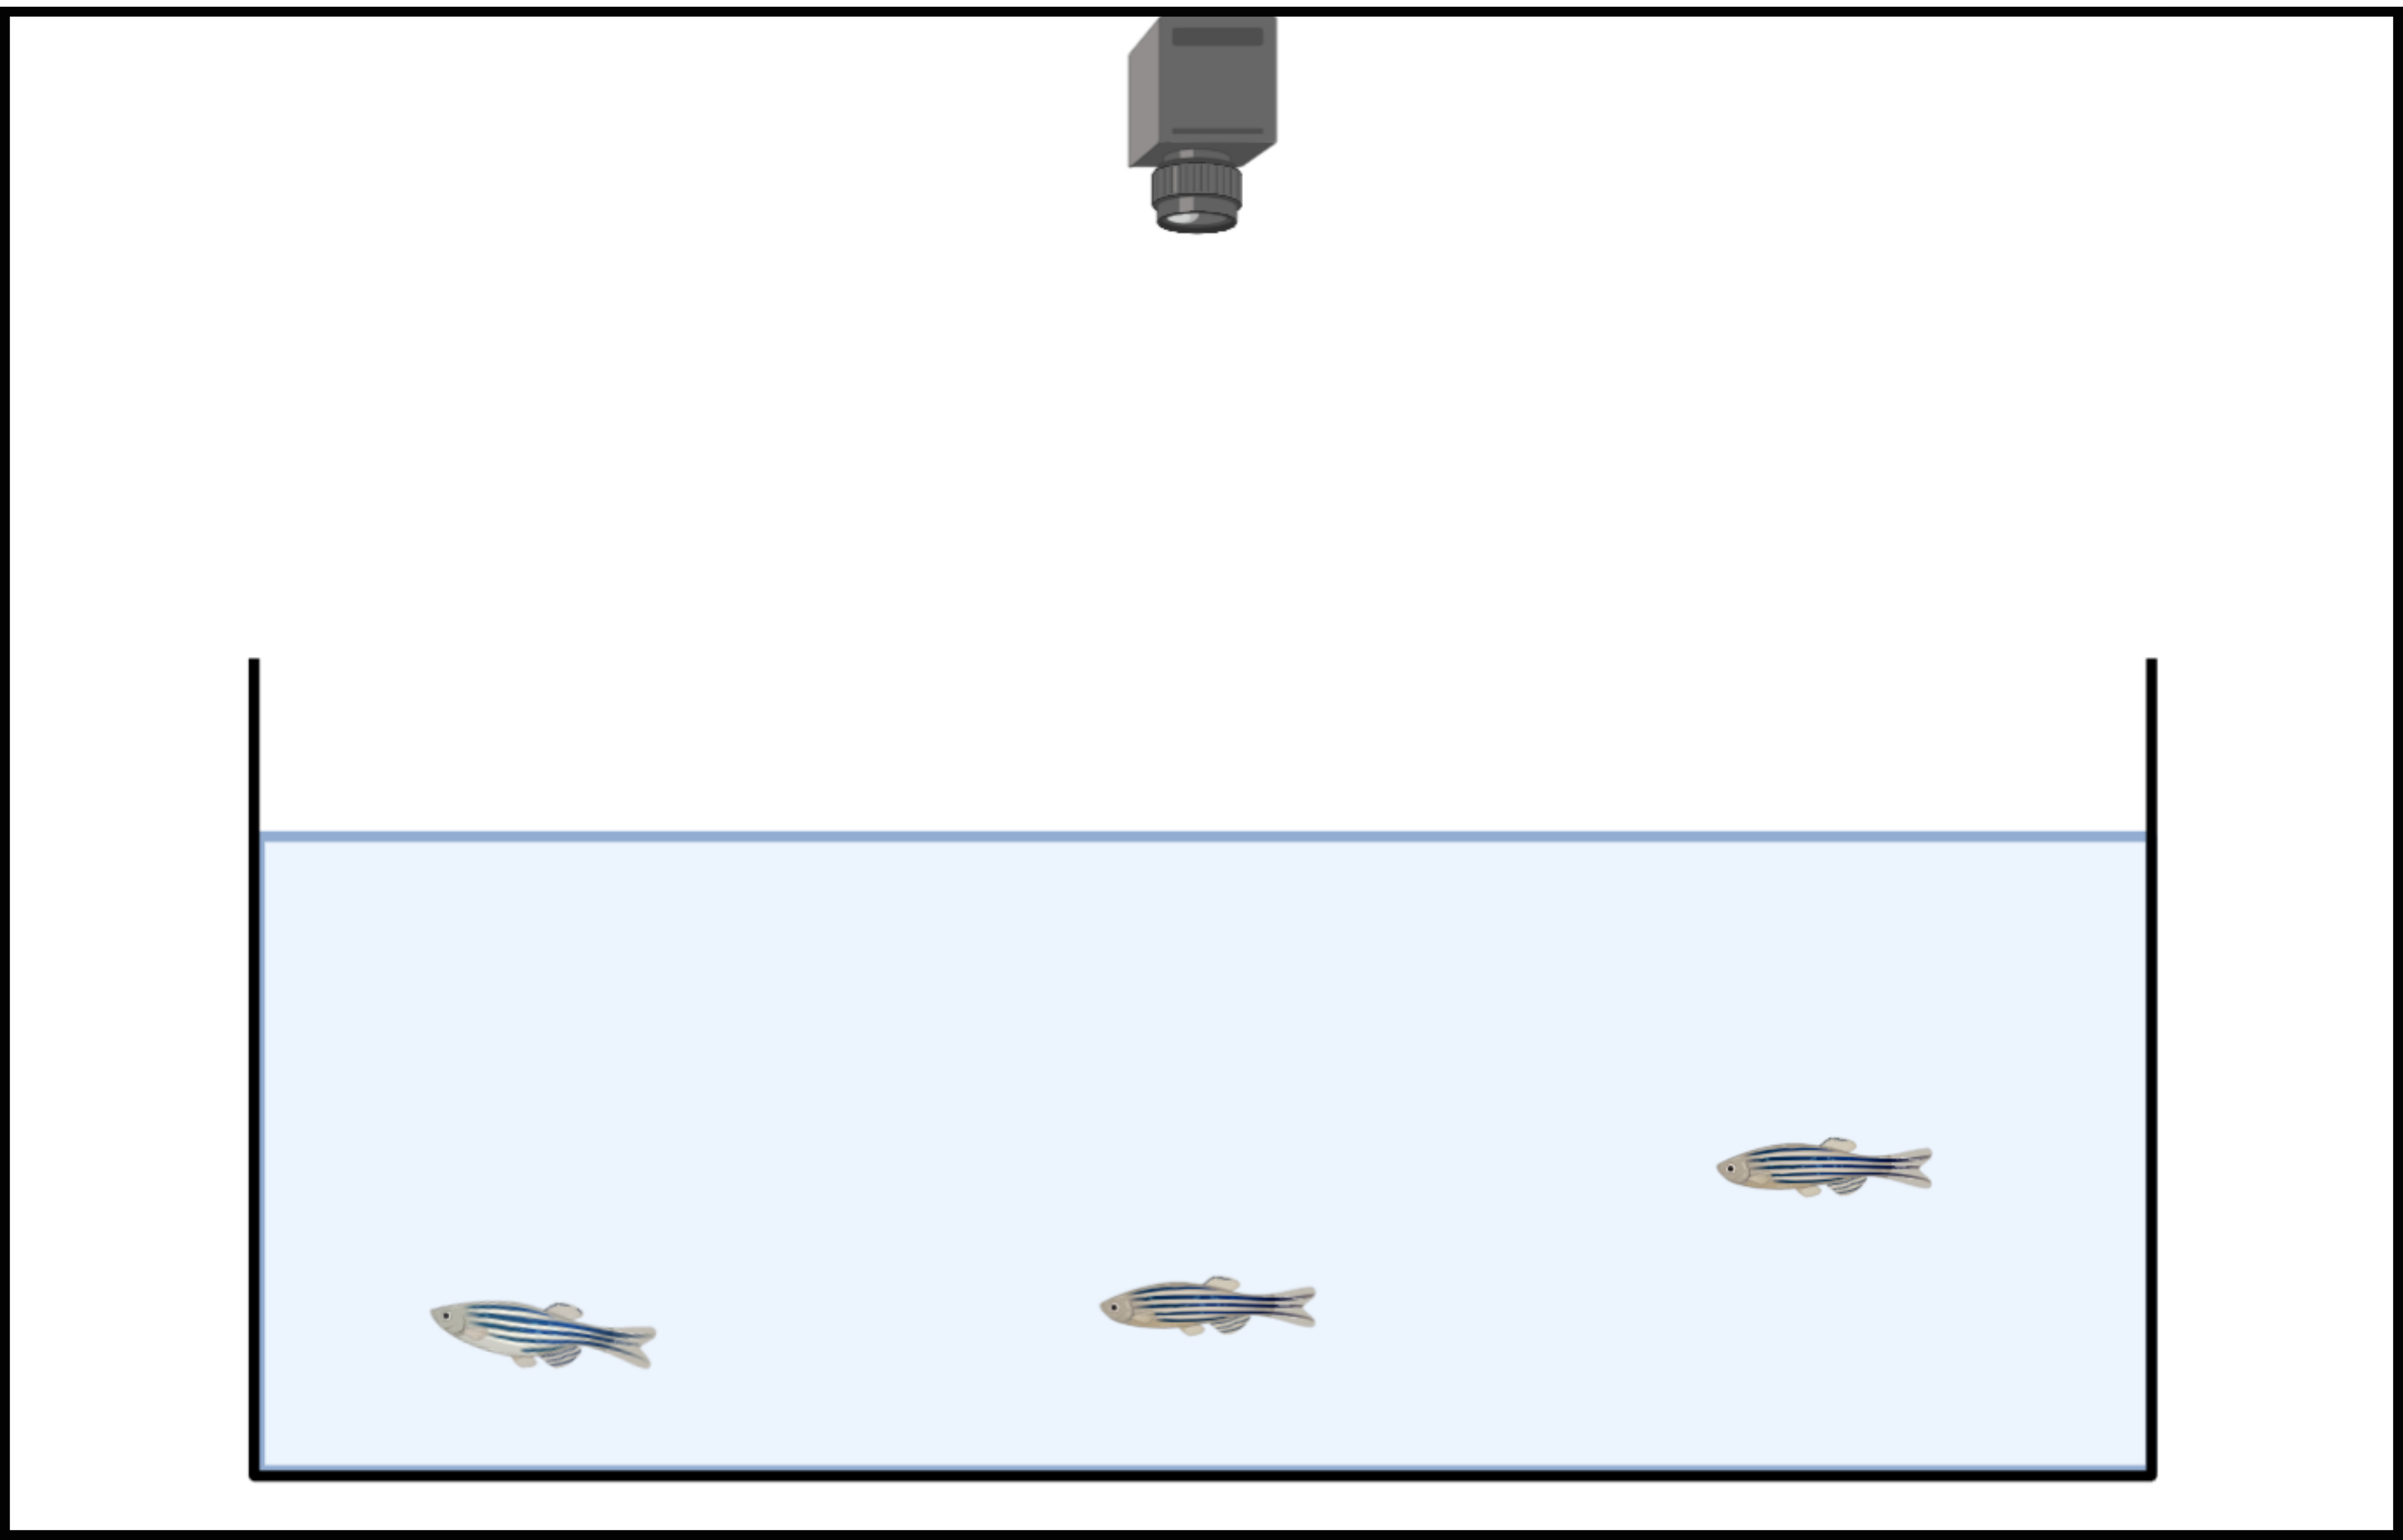
\includegraphics[width=0.6\textwidth]{recording}
	\caption{Video recording setup}
	\label{fig:recording}
\end{figure}

\subsection{Annotating Data}
The data is annotated with bounding boxes for object detection. Annotations are made using the \textit{labelme} Python annotation tool \citep{labelme2016}. A snapshot of the UI of the software is shown in \autoref{fig:labelme}.

\begin{figure}[H]
	\centering
	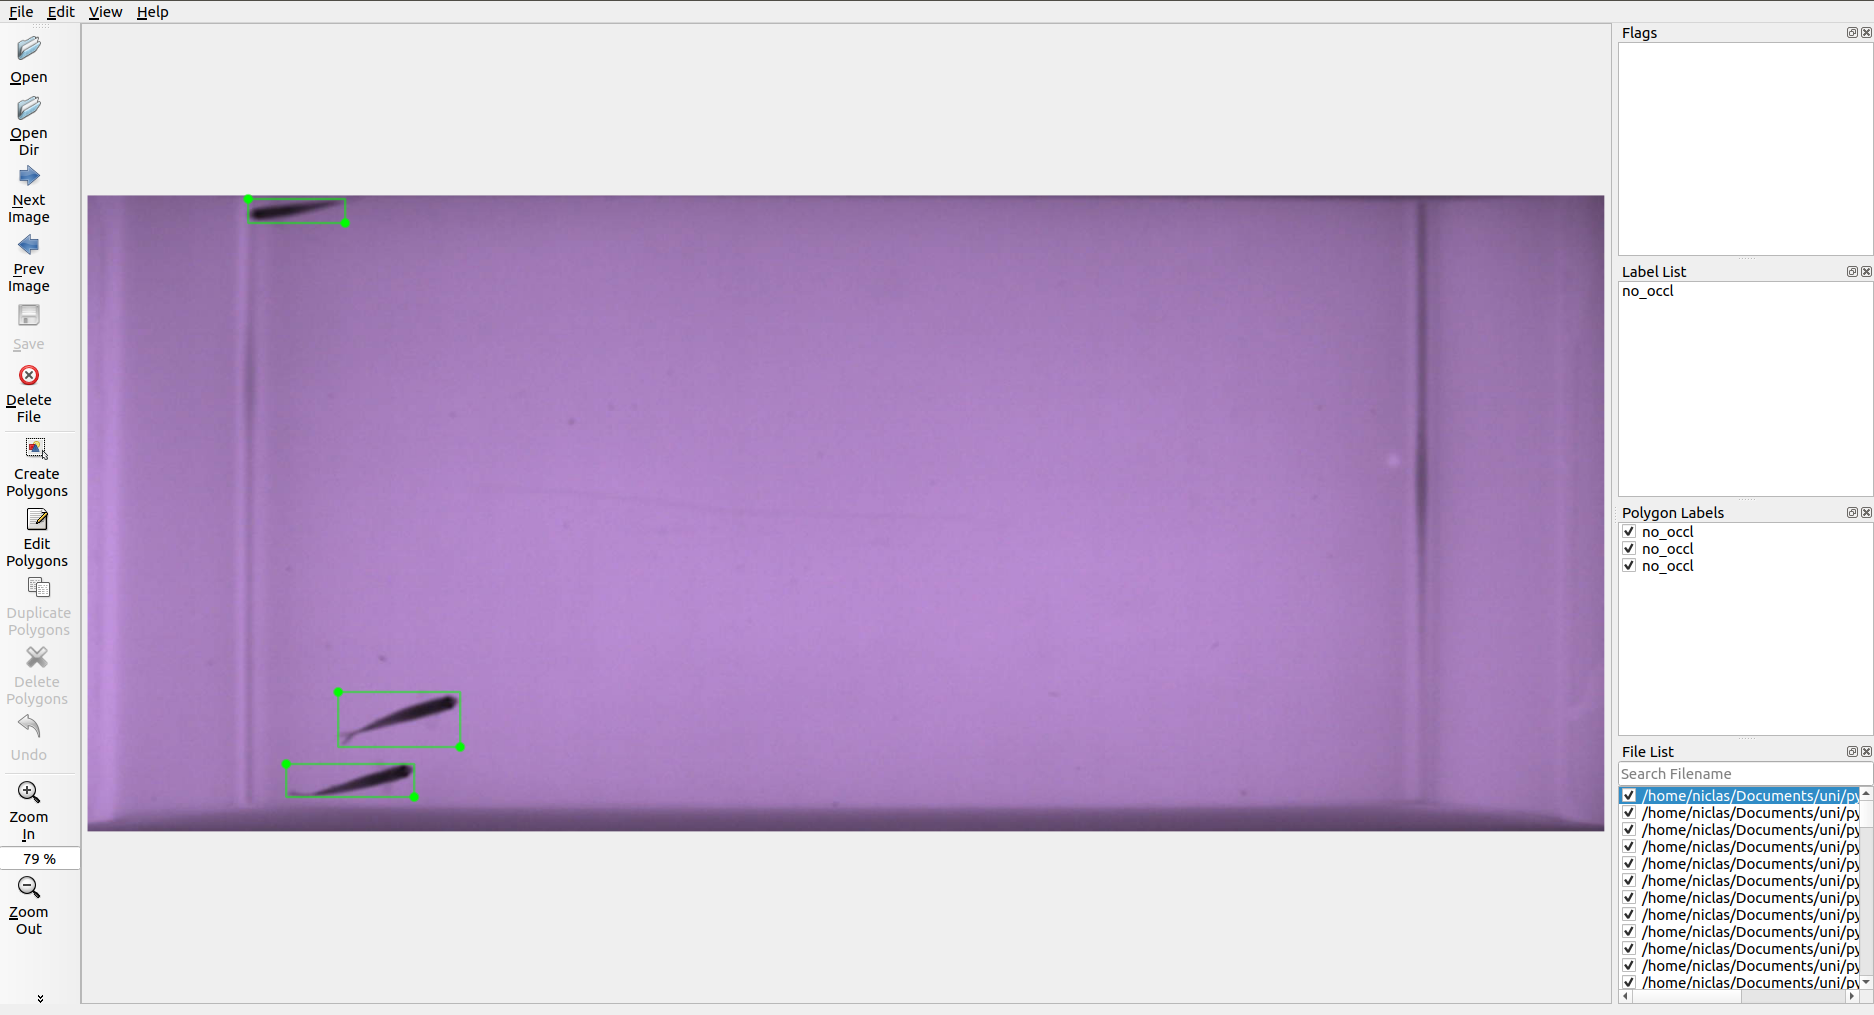
\includegraphics[width=0.8\textwidth]{labelme}
	\caption{Snapshot of labelme annotation tool while annotating data}
	\label{fig:labelme}
\end{figure}

The software is able to export annotations in formats matching both VOC PASCAL and COCO, which is either an XML-file for each image using the VOC PASCAL annotation style or a json file using the COCO annotation style. The file-type chosen is the PASCAL VOC XML-files, with individual files for each image annotated.\\

The annotations are made up of both \textit{no occlusions} and different types of occlusions presented in the following section.

\section{Fish Shapes}
Even a single zebrafish is able to twist into many different shapes, according to \cite{Kalueff2013} zebrafish has an extensive catalogue of behavioural patterns, which are also based on different contortions of the body. The main shapes of a single zebrafish are shown in \autoref{fig:single_shape}. The shapes shown are only the ones seen from the top view of an aquarium.

\begin{figure}[H]
	\centering
	\begin{subfigure}[b]{0.3\textwidth}
		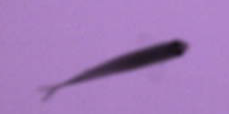
\includegraphics[width=\textwidth]{straight}
		\caption{Zebrafish lying completely straight}
		\label{fig:straight_fish}
	\end{subfigure}
	\begin{subfigure}[b]{0.3\textwidth}
		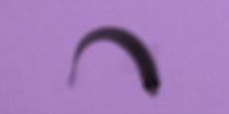
\includegraphics[width=\textwidth]{c-shape}
		\caption{Zebrafish creating a C shape}
		\label{fig:c-shape_fish}
	\end{subfigure}
	\begin{subfigure}[b]{0.3\textwidth}
		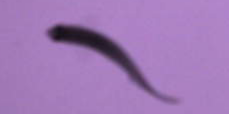
\includegraphics[width=\textwidth]{s-shape}
		\caption{Zebrafish creating an S shape}
		\label{fig:s-shape_fish}
	\end{subfigure}
\caption{Different shapes a zebrafish makes from a top view, also described by \cite{Kalueff2013}}
\label{fig:single_shape}
\end{figure}

\cite{Kalueff2013} states that the C-shape is made as starting movement to propel itself forward, often in order to escape or because the zebrafish is startled. The bending into a C-shape, can also be caused by the zebrafish turning. The S-shape is made for the same reasons as the C-shape, to propel the zebrafish forward.\\

When two zebrafish are touching or crossing each other in any way, they create multiple new shapes.

\subsection{Touching}
When two zebrafish are touching they in general create three different kind of shapes. They will either be elongating one another, creating one single long object. This can be either head-to-head, tail-to-tail, or head-to-tail. Two examples are shown in \autoref{fig:elongation}. When touching head-to-tail it is most often seen as courtship between a male and a female zebrafish \citep{Kalueff2013}.

\begin{figure}[H]
	\centering
	\begin{subfigure}[b]{0.47\textwidth}
		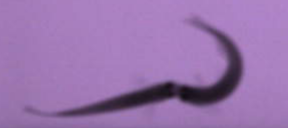
\includegraphics[width=\textwidth]{headhead}
		\caption{Head-to-head elongation}
		\label{fig:headhead}
	\end{subfigure}
	\begin{subfigure}[b]{0.47\textwidth}
		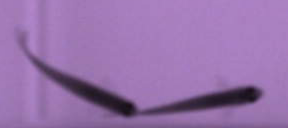
\includegraphics[width=\textwidth]{headtail}
		\caption{Head-to-tail elongation}
		\label{fig:headtail}
	\end{subfigure}
\caption{The two touching possibilities creating an elongation}
\label{fig:elongation}
\end{figure}

Two zebrafish touching is done in all kinds of positions and angles. When touching end-to-end but at a tighter angle, two zebrafish tend to create a V-shape. In the beginning and end of a crossing or when touching the head or tail to the middle of the body of another zebrafish, a T-shape is created. Examples of both shapes are shown in \autoref{fig:TandV}.

\begin{figure}[H]
	\centering
	\begin{subfigure}[b]{0.47\textwidth}
		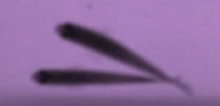
\includegraphics[width=\textwidth]{v-shape}
		\caption{V-shape created by two zebrafish touching tails}
		\label{fig:v-shape}
	\end{subfigure}
	\begin{subfigure}[b]{0.47\textwidth}
		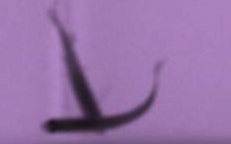
\includegraphics[width=\textwidth]{t-shape}
		\caption{T-shape example}
		\label{fig:t-shape}
	\end{subfigure}
\caption{Examples of V- and T-shape}
\label{fig:TandV}
\end{figure}

\subsection{Above and Below}
More complex occlusions often happen when one zebrafish is above the other. The water depth of the aquarium affect this as the zebrafish are more likely to swim above each other if the water depth allows for it. There is mainly two different occlusions happening in this instance; two zebrafish creating a cross or one zebrafish almost completely occluding the other.

The crossing can happen in multiple angles. A crossing occlusion is defined as two zebrafish creating an X-shape. Examples of different crosses are shown in \autoref{fig:cross}. 

\autoref{fig:crossWide} shows a crossing occlusion, which is close to being an \textit{on-top} occlusion, but will be defined as a cross due to the head and tails being separated.

\begin{figure}[H]
	\centering
	\begin{subfigure}[b]{0.3\textwidth}
		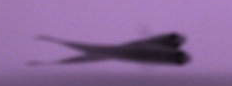
\includegraphics[width=\textwidth]{crossWide}
		\caption{Cross occlusion at a wide angle}
		\label{fig:crossWide}
	\end{subfigure}
	\begin{subfigure}[b]{0.3\textwidth}
		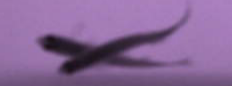
\includegraphics[width=\textwidth]{crossSemi}
		\caption{Cross occlusion at a semi-wide angle}
		\label{fig:crossSemi}
	\end{subfigure}
	\begin{subfigure}[b]{0.3\textwidth}
		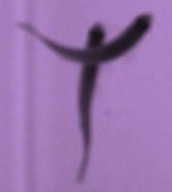
\includegraphics[width=\textwidth]{crossRight}
		\caption{Cross occlusion at an almost right angle}
		\label{fig:crossRight}
	\end{subfigure}
	\caption{Different cross occlusions}
	\label{fig:cross}
\end{figure}

The on-top occlusions is when one zebrafish is somewhat straight on top of another zebrafish. This kind of occlusions can, at times, be a shorter kind of elongation e.g. when the head of the top zebrafish is further in on the body of the bottom zebrafish. Examples of op-top occlusion are shown in \autoref{fig:onTop}.

\begin{figure}[H]
	\centering
	\begin{subfigure}[b]{0.47\textwidth}
		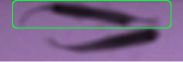
\includegraphics[width=\textwidth]{onTop}
		\caption{Straight on top occlusion of two zebrafish}
		\label{fig:onTopFull}
	\end{subfigure}
	\begin{subfigure}[b]{0.47\textwidth}
		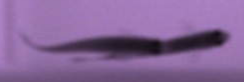
\includegraphics[width=\textwidth]{onTopMid}
		\caption{Head on top of middle of bottom zebrafish}
		\label{fig:onTopMid}
	\end{subfigure}
	\caption{On-top occlusions by two zebrafish}
	\label{fig:onTop}
\end{figure}

\subsection{Other Occlusions}
Besides the five previously mentioned types of occlusions, several other occlusions occur which are harder to classify as they do not fall into any specific category. Due to this, a category named \textit{other} is created as well. Some examples of these kinds of occlusions are shown in \autoref{fig:other}.

\begin{figure}[H]
	\centering
	\begin{subfigure}[b]{0.3\textwidth}
		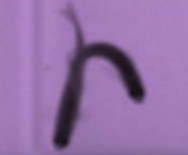
\includegraphics[width=\textwidth]{otherR}
		\caption{Example of occlusion categorised as \textit{other}}
		\label{fig:otherR}
	\end{subfigure}
	\begin{subfigure}[b]{0.3\textwidth}
		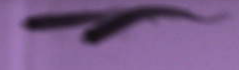
\includegraphics[width=\textwidth]{otherTop}
		\caption{Example of occlusion categorised as \textit{other}}
		\label{fig:otherTop}
	\end{subfigure}
	\begin{subfigure}[b]{0.3\textwidth}
		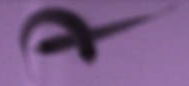
\includegraphics[width=\textwidth]{otherP}
		\caption{Example of occlusion categorised as \textit{other}}
		\label{fig:otherP}
	\end{subfigure}
	\caption{Different \textit{other} occlusions}
	\label{fig:other}
\end{figure}

Occlusions occurring with all three zebrafish are also categorised as other, as none of these fall into the defined categories, but are still occlusions.

The more zebrafish included in an occlusion the higher the complexity of the occlusion is prone to be. This includes both the type of occlusion occurring between each pair of the zebrafish but also possible occlusions and crossings of multiple zebrafish occurring at the same time. 
At some occasions, a three zebrafish occlusion is easily split into two different types of occlusions and all three zebrafish are very distinguishable from one another, as in \autoref{fig:3f_EC}, but at other times three zebrafish will stack upon each other as in \autoref{fig:3f_stack}.

\begin{figure}[H]
	\centering
	\begin{subfigure}[b]{0.47\textwidth}
		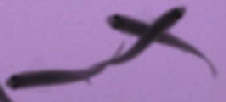
\includegraphics[width=\textwidth]{3f_occl_EC}
		\caption{Three zebrafish in distinguishable occlusions}
		\label{fig:3f_EC}
	\end{subfigure}
	\begin{subfigure}[b]{0.47\textwidth}
		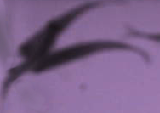
\includegraphics[width=\textwidth]{3f_stack}
		\caption{Three zebrafish in a stacking occlusion}
		\label{fig:3f_stack}
	\end{subfigure}
	\caption{Occlusions amde by three zebrafish}
	\label{fig:3fish_occl}
\end{figure}

As can be seen in \autoref{fig:3fish_occl}, the occlusions occurring are either combinations of the occlusions with only two zebrafish or the same type of occlusion multiple times. Due to this it is chosen to focus on the occlusions occurring between two zebrafish and prove feasibility of this to be able to, later, expand a solution to handle occlusions with more than two zebrafish.

\section{Occlusion Frequency}
In the data set the occlusions happen with different frequencies. The frequencies are displayed in a bar chart in \autoref{fig:occlFreq}.

\begin{figure}[H]
	\centering
	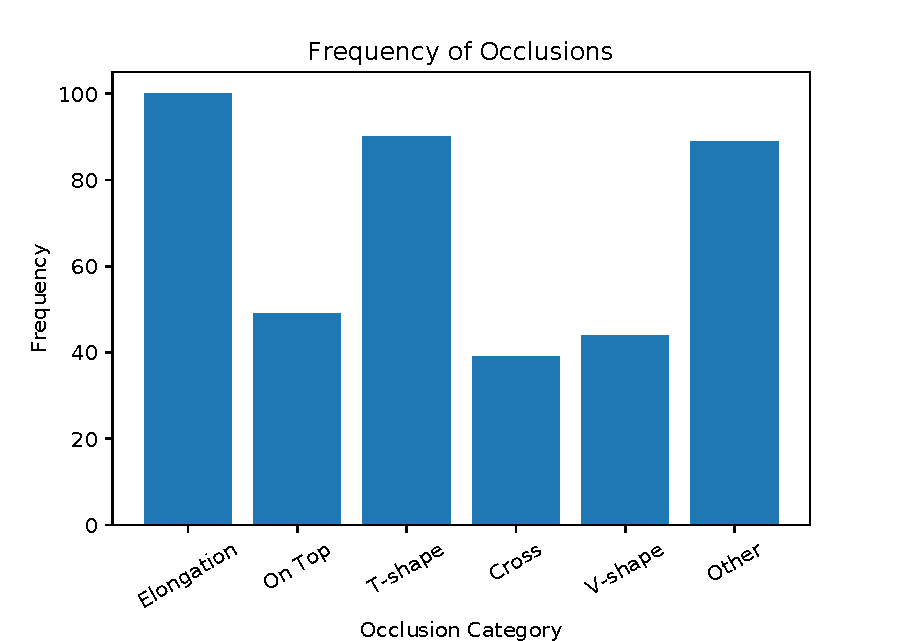
\includegraphics[width=0.8\textwidth]{occlFreq}
	\caption{Frequency of the different types of occlusions}
	\label{fig:occlFreq}
\end{figure}

\autoref{fig:occlFreq} shows that elongation is the most frequently occurring occlusion, together with the T-shape and other types of occlusions. In total $ 411 $ occlusions occur out of $ 3000 $ frames, which is a frequency of $13.7\%$.